\documentclass[11pt,a4paper,oneside]{article}

\usepackage[english,russian]{babel}
\usepackage[T2A]{fontenc}
\usepackage[utf8]{inputenc}
\usepackage[russian]{olymp}
\usepackage{hyperref}
\usepackage{graphicx}
\usepackage{expdlist}
\usepackage{mfpic}
\usepackage{amsmath}
\usepackage{amssymb}
\usepackage{comment}
\usepackage{listings}
\usepackage{epigraph}
\usepackage{url}
\usepackage{ulem}
\usepackage{placeins}

\DeclareMathOperator{\nott}{not}

\begin{document}

\renewcommand{\t}[1]{\mbox{\texttt{#1}}}
\newcommand{\s}[1]{\mbox{``\t{#1}''}}
\newcommand{\eps}{\varepsilon}
\renewcommand{\phi}{\varphi}
\newcommand{\plainhat}{{\char 94}}

\newcommand{\Z}{\mathbb{Z}}
\newcommand{\w}[1]{``\t{#1}''}

\binoppenalty=10000
\relpenalty=10000

\createsection{\Note}{Комментарий}

\contest{The article for the master thesis, draft}{Dmitry Filippov}{August 1, 2018}

\center{\textbf{Finding the subgraphs of the social graph containing the given users}}

\chapter{Introduction}

Maybe something need to be written here

%%%%%%%%%%%%%%%%%%%%%%%%%%%%%%%%%%%%%%%%%%%%%%%%%%%%%%%%%%%%%%%%%%%%%%%%%%%%%%%%%%%%%%%%%%%%%%

\section{Terms and definitions}

\subsection{Graph terms}

In this chapter we will write down all non-common terms and definitions that may be helpful for the further reading.


Under \textbf{$N_G(v)$} we will understand the set of the neighbors of vertex $v$ in graph $G$, i.e. the set of the vertices that are directly connected to $v$ by edge: $N_G(v) = \{u | (v, u) \in E(G)\}$. If graph $G$ can be obviously recognized from the context, we can write just $N(v)$.

\textbf{$G[V]$} is called \textbf{originated subgraph} of the graph $G$ by the set of vertices $V$ if $G[V] := (V, E[G, V])$, where $E[G, V]$~--- the subset of the set of edges of $G$, both ends of which are contained in $V$, i.e. $E[G, V] = E(G) \cap (V \times V)$.

\textbf{k-truss} of the graph $G$ is the subgraph $G' \subseteq G$ containing the maximal possible number of vertices, such that for each edge $(v, u)$ the number of vertices $w$, such that edges $(w, v)$ and $(w, u)$ exists in $G'$ is at least $k$. In other words, $k-truss$ is the maximal by size subgraph $G'$, for each of which edge $(v, u)$, the $|N_{G'}(v) \cap N_{G'}(u)| >= k$ is true.

\textbf{k-core} of the graph $G$ is called the maximal by the number of vertices subgraph $G' \subseteq G$, so that the degree of each of its vertices is at least $k$. For the fixed $k$, by $C_k$ we will denote \textit{$k$-core}, namely the set of the connected components of which it consists. So, $C_k = \{H_i\}$, where $H_i$ is the $i$-th connected component, where the degree of each vertex is at least $k$. The number $k$ we will call the \textbf{order} of \textit{k-core}.

By \boldmath$\mu(G)$\unboldmath we will denote the minimal degree of the vertices $G$, i.e. $\mu(G) = \min_{v \in V(G)} deg(v)$.

\textbf{Core decomposition} is the set of \textit{k-core} for all possible $k$: $C = \{C_k\}_{k=1}^{k=k^*}$. We also need to clarify that from the definition of the \textit{k-core} you can see that $C_1 \supseteq C_2 \supseteq C_3 \ldots \supseteq C_{k^*}$ (where $k^*$ is the maximal possible $k$ in core decomposition).

\textbf{Сore index} for the vertex $v$ is called the minimal by the size \textit{k-core} which includes $v$, i.e. \textit{k-core} with the maximal $k$: $c(v) = \max(k \in [0..k^*] | v \in C_k)$.

\textbf{$\gamma$-quasi-clique} of the graph $G$ is called any such subgraph $G' \subseteq G$ that it is <<dense enough>>, i.e. $\frac{2 \cdot |E(G')|}{|V(G')| \cdot (|V(G')| - 1)} \ge \gamma$.

\subsection{Social networks}

\textbf{The community} or \textbf{The community in social network} is called the set of vertices of the social network $G$, where all vertices are united by some property or attribute. For example, <<the community of rock lovers>> or <<the community of Apple shareholders>>.

\textbf{The social clique} or \textbf{clique} we will call the set of people in social network, where everyone "knows" (i.e. is connected by edge) each other, in other words when between any pair of distinct people there is an edge in social network.

\textbf{Social pseudoclique} or \textbf{pseudoclique} we will call the set of people, where it is not required that each pair of distinct people is connected by edge, but this set is still densely connected. The estimation, how dense the pseudoclique is connected depends on the type of the pseudoclique and will be discussed later in the work, but in all definitions the biggest role plays the number of edges in subgraph in comparison with the number of pairs of vertices ($\frac{2 \cdot |E(G)|}{|V(G)| \cdot (|V(G)| - 1)}$).

\textbf{Free-rider effect} is called the effect, appearing during the obtaining the answer for the given task (finding the dense community in social network), when the final or intermediate answer contains unnecessary subgraphs~--- subgraphs which can be deleted without violation the optimality of the answer. Thereby, we can make the answer smaller which is one of ours main goals.

\subsection{Useful abbreviations}

\textbf{RW}~--- Random Walks. The main idea of this method is based on moving from one vertex to the neighbor one with probability proportional to the edge weight.

\textbf{RWR}~--- Random Walks with Restarts. The idea is similar to the RW, but in this case the probability to move to the initial vertex (from which we've started) from the current one exists as well.

\textbf{Smart-ST}~--- Smart Spanning Trees. The heuristic for Steiner Tree problem, which is used in Gionis et al. article \textbf{[1]}.

\textbf{CSP}~--- Community Search Problem. This is the task for finding the community in the social network which contains all the selected vertices.

\textbf{NCSP}~--- Noising Community Search Problem. This is the task for finding the community in the social network which contains most of the selected vertices, but not necessary all (not including the noise).

\section{Overview}

The task that we're analyzing in the work is formulated as follows: given a graph $G$ and a set of selected vertices $Q \subset V(G)$, the goal is to solve community search task~--- to find the community which contains most of the vertices from $Q$, but not necessary all of them. Sometimes we will call vertices from $Q$ <<query vertices>>, <<query>> or <<vertices from query>>.

\subsection{Initial solutions}

\begin{enumerate}
  \item The community search task by the given selected vertices is researched during a long time. Even in 2004 Faloutsos et al. \textbf{[2]} suggested the algorithms for finding the dense community by $2$ selected vertices in network ($|Q| = 2$). The algorithm shows that metrics like <<the shortest path>> and <<max flow>> between two given vertices are not optimal. Instead of them, the initial graph is considered as the electric network and <<the current delivered between vertices>> metric is used~--- setting voltage \texttt{+1} on the first vertex-query and \texttt{0} on the second one, we find subgraph which delivers the maximal current between vertices from query. The provided metrics works only for $|Q| = 2$, but this algorithm was the foundation in research of the community search task. After that many authors were working on optimization for this article and were quite successful.

  \item Authors of the second article that was taken for consideration \textbf{[3]} suggest the metric function based on \textit{random walks with restarts} (RWR) used on the weighted graph. They consider $r(i, j)$~--- the probability that starting in vertex $i$-th query vertex $q_i$ we will end in vertex $j$ using RWR, where on each step we move to the neighbor by edge vertex with probability proportional the edge weight. Also we introduce $r(Q, j)$ which is equal to the sum of $r(i, j)$ for each query vertices: $r(Q, j) = \sum_{i = 1}^{i = |Q|}\; r(i, j)$. The dense metric is considered as $g(H) = \sum_{j \in H}\; r(Q, j)$. This method has shown quite good results compared to the previous article, because expanded the number of query vertices from $2$ to any number from $2$ to $|V(G)|$. Also, it introduced new ability of finding the subgraph containing not all vertices, but at least $k$ of them ($k$ is a parameter which is given as input). This operation was called $K\_softAND$ and was successfully implemented in the article. Further algorithms were expanding this idea, were applying other metrics and improved the results of this algorithm, but the task of finding the community containing not necessary all query vertices, but only a part of them (our task), almost wasn't optimized.

  \item Authors of the third article \textbf{[4]} suggest to use \textit{Wiener index} as the metric for subgraph density. This metric is equal to the pairwise sum of the shortest distances between vertices from the query. Authors are trying to solve the issue of obtaining too large graph as the result of processing the query if query vertices are placed in several communities and are weakly connected between each other. To solve this issue, authors suggest to add some <<important vertices>> to the query which will connect communities, even if not very dense. Results has shown that this method works several times better than previous methods \textbf{[1, 3]} and almost the same as the methods that based on \textit{Steiner tree problem}. Unfortunately, the article doesn't consider more late methods based on \textit{Steiner tree problem} which significantly improved the old results, which make this method less priority comparing to them.
  
\end{enumerate}

\subsection{Finding optimal pseudocliques}

The most part of all algorithms for solving the described task are the algorithms based on the finding optimal pseudocliques with some additional heuristics. There are a lot of different pseudocliques the were considered in different articles: for example, \textit{k-core} \textbf{[5]}, \textit{$\gamma$-quasi-clique} \textbf{[6]} or just algorithms that maximizes the edge density in the resulting subgraph \textbf{[7]} which is almost a definition of a pseudoclique. For each of these pseudocliques the algorithms are evolving and becoming better, optimizing the previous results using new heuristics. Comparing the results of the algorithms that use different pseudocliques is quite hard and unlikely will give visible results because of the difference of the metrics that are being optimized~--- the result strongly depend on the initial graph and the queries on it. In some cases one pseudoclique will obtain results better than others, but in other cases it will work worse, so actually it's worth to compare some common performance metrics, but unfortunately it doesn't give us the whole understanding of the optimality or non-optimality of the algorithms.

Let's consider several newest algorithms for the most popular pseudocliques:

\begin{enumerate}
  \item X. Huang et al. \textbf{[8]} choose \textit{k-truss} pseudoclique. However, just finding the optimal \textit{k-truss} (i.e. \textit{k-truss} with the maximal $k$ containing all query vertices in it) is not an optimal solution, and also it is an already solved problem (even with polynomial solution). That's why the authors of the article suggest to find \textit{k-truss} with maximal $k$ and minimal subgraph diameter, which, as they show in their article, is a NP-hard problem. However, this idea pretends to show good results, so authors made a research trying to understand how close the answer found by polynomial time may be to the theoretically optimal answer. It turned out that this problem couldn't be solved with accuracy better than in $(2 - \varepsilon)$ times worse for each $\varepsilon > 0$ (under the accuracy we understand the length of the diameter in the final answer). However, authors suggested the heuristic algorithm which in the worst case makes exactly $2$ times error, which shows that their algorithm is optimal for the provided problem. The algorithm is based on building the supposed maximal $\textit{k-truss}$ with the followed iterative deleting vertices which doesn't make the answer worse and make the diameter smaller. The results obtained in this article are really good comparing to the previous articles \textbf{[7, 9]}, however, even despite of proved optimality for the provided algorithm, it is not optimal for the initial problem (finding the dense subgraph by the given query vertices), because authors found the optimal solution only for the problem provided \textit{by themselves}.

  
  \item N. Barbieri et al. \textbf{[5]} is using \textit{k-core} pseudoclique. However, even here simple finding the optimal \textit{k-core} (i.e. \textit{k-core} with maximal $k$ which contains all query vertices in it) is not an optimal solution, and also this problem is already solved by polynomial time \textbf{[9]}. That's why the authors of the article apply some heuristics targeted for minimizing the size of the resulting subgraph without loosing its optimality. These heuristics allow to reduce the problem to finding the answer in component $H^* \subset G$, and besides it is guaranteed that all possible optimal answers for the initial problem are lying in $H^*$. After that authors bring some heuristics for minimizing the obtained subgraph $H^*$. The main statement described by the authors is not new, but it looks quite interesting for the further researches because it adds more information to the initial problem without loosing any solutions. The results of this article shows that provided method really works better and faster than previous ones \textbf{[9, 10]}. Based on all the above information, it was decided to take this article as the baseline and try to improve it, especially to expand it to our problem (finding the community containing not necessary all selected vertices).
\end{enumerate}

\subsection{Other methods}

As we already saw earlier, optimizing functions may be quite different. In the previous part we were considering pseudocliques, and here we're going to consider several other popular optimizing functions.

\begin{enumerate}
  \item L. Akoglu et al. \textbf{[11]} slightly change the initial problem~--- they try to find subgraph that unites not all the vertices in the query, but their groups. Actually the idea is based on splitting the query into groups and building the answer for each of the groups separately, so that in each groups the vertices are densely connects and are united by some common property. But between each other the groups may be connected not very densely. This corresponds to the splitting the query into several communities. The results of the article has shown that this method solves the problem provided by authors quite good, but however as we said before, this task differs from ours and it's hard to compare it's results with ours. However, we still are going to compare this solution with ours, because this solution supports finding community not for all selected vertices. 

  \item A. Gionis et al. \textbf{[1]} in their article consider \textit{linear local discrepancy} metric which is equal to the weighted difference of the number of query vertices in the resulting subgraph and the number of remaining vertices. More formally, $g(C) = \alpha p_C - n_C$, where $p_C = |Q \cap V(C)|$ and $n_C = |V(C) \setminus Q|$. The algorithm that maximized this function based on the \textit{Steiner tree problem} and \textit{Smart-ST}s. The distinguishing feature of this algorithm is the ability of solving the problem using \textit{local access model}, i.e. the model where we don't know the whole graph (or it is too big to save it in RAM), and API allows us only to make queries for accessing all vertex neighbors~--- $get-neighbors$ method. This model allows to solve the problem optimally even on very big social networks, such as \textit{Twitter} or \textit{Facebook}. Based on the definition, the resulting subgraph may not contain all vertices from query, which coincides with our research. Unfortunately, the provided metric doesn't fit our problem very good~--- it doesn't take into consideration edge density of the resulting subgraph, it looks only the ratio of the vertices. Also it's possible that the answer will contain too few vertices from the initial query~--- it also doesn't work for us.
\end{enumerate}

\section{Final requirements for our work}

Let's sum up everything described above. Most of the current solutions solves CSP quite optimal~--- each of the solutions uses it's own metric and obtains quite good results. However, as we can see, solutions for NCSP (which includes noise into consideration) are quite rare, despite it is more useful problem in real life. We've noted consideration of NCSP problem in articles C. Faloutsos \& H. Tong \textbf{[3]} and A. Gionis et al. \textbf{[1]}, however the last problem is not based on solving NCSP (but solves it at the same time). So, the goal of our article will be to build the algorithm that focuses on NCSP solving and obtains better results than the current ones. Here are some requirements for our algorithm:

\begin{itemize}
    \item The algorithm should obtain better results than the current ones \textbf{[1, 3, 5]};
    \item The algorithm should be quite optimal, ideally not loosing the competition with other algorithms in terms of working time;
    \item It would be an advantage to support backwards compatibility~--- if the user wants to find subgraph that contains \textit{all} query vertices, it should be possible to be done.
\end{itemize}

%%%%%%%%%%%%%%%%%%%%%%%%%%%%%%%%%%%%%%%%%%%%%%%%%%%%%%%%%%%%%%%%%%%%%%%%%%%%%%%%%%%%%%%%%%%%%%%%%%%%%%%%%%%%%%%%%%%%%

\thechapter{Suggested algorithm}

Для решения нашей задачи нужно для начала разобраться с двумя вопросами:

\begin{enumerate}
  \item Как оценивать плотность итогового подграфа?
  \item Что такое <<большинство вершин-запросов>>?
\end{enumerate}

Для сравнения подгафов, полученных разными алгоритмами мы будем использовать реберную плотность и размер итогового подграфа: $density(G) = \frac{2 \cdot |E(G)|}{|V(G)| \cdot (|V(G)| - 1)}$, $size(G) = |V(G)|$. Действительно, если ребер в полученном подграфе достаточно много, можно считать, что он плотный. Однако также хочется, чтобы при этом он имел как можно меньший размер. Что же такое <<большинство вершин-запросов>> в подграфе-ответе мы обсудим чуть позже.

\section{Описание идеи алгоритма}

Так как алгоритмов, решающих именно нашу задачу, слишком мало, у нас есть два подхода к решению поставленной задачи~--- придумать полностью новый алгоритм или усовершенствовать один из существующих, требующих наличие всех вершин-запросов в ответе. Далее для описания задачи поиска сообщества, содержащего все выделенные вершины-запросы мы будем использовать сокращение \textit{CSP}, а для нахождения сообщества, содержащего большинство вершин-запросов~--- \textit{NCSP}.

Полностью новым алгоритмом будет, например, следующий: перебрать множество вершин, которое по нашему мнению является шумом, найти подграф, содержащий все остальные вершины одним из существующих алгоритмов, требующих наличие всех вершин-запросов, а затем обновить ответ. Это решение имеет место быть и даже будет выдавать наиболее оптимальный ответ, однако понятно, что это слишком долго~--- перебор множества игнорируемых вершин будет иметь экспоненциальную от их количества асимптотику, которая затем умножается еще и на асимптотику выбранного алгоритма, ищущего CSP для оставшихся вершин. Поэтому мы не будем использовать этот метод, а попытаемся предложить что-нибудь другое.

Более простым путем будет усовершенствование идеи одного из последних алгоритмов, решающих CSP. Действительно~--- идея (что именно оптимизировать) уже проверена и показала неплохие результаты, и если применить другие эвристики, которые позволят учитывать постановку нашей задачи, может получиться неплохой результат. Так мы и сделаем: возьмем алгоритм Barbieri et al. \cite{Barbieri15} и попробуем его расширить на нашу задачу. Статьи Bogdanov et al. \cite{Bogdanov13} и Cui et al. \cite{Cui14} показали, что максимизация минимальной степени вершины является эффективным способом нахождения оптимального сообщества, поэтому наша идея имеет место быть. 

Идея алгоритма Barbieri et al. \cite{Barbieri15} заключается в нахождении в графе $G$ \textit{k-core} с максимальным $k$, а также минимального размера, содержащим все вершины из $Q$. В статье авторы показывают, что это NP-полная задача, а следовательно для ее решения нужны эвристики. Это не является плохой стороной, потому что на данный момент не существует алгоритмов, в которых задача, оптимизируемая для поиска оптимального сообщества, является решаемой за полиномиальное время, а сами алгоритмы показывают хорошие результаты. Так, например, Sozio et al. \cite{Sozio10} ищут \textit{k-core} с максимальным $k$, не обращая внимание на минимальность его размера. Эта задача оказывается решаемой за линейное время от количества ребер в графе, однако, этот алгоритм выдает слишком большие подграфы. Введение же параметра $size$, ограничивающего размер итогового подграфа сразу делает задачу NP-полной, что авторы и показывают в статье.

Возвращаясь к статье Barbieri et al. \cite{Barbieri15}, отметим главную идею их алгоритма. Алгоритм опирается на следующее утверждение: если взять ядерную декомпозицию $C = \{C_k\}_{k=1}^{k=k^*}$ графа $G$, а затем найти такое максимальное $k'$, что все вершины из запроса $Q$ лежат в одной и той же компоненте $H^* \in C_{k'}$, то все ответы на CSP находятся в этой компоненте $H^*$. Более формально: $k' = \max\{k | \exists H_i\mbox{~--- компонента связности } C_{k'}\mbox{, т.ч. } \forall v \in Q: v \in H_i\}$. Найденный \textit{k-core} мы будем обозначать $C_Q^*$, а компоненту, содержащую все вершины из $Q$~--- $H^*$. Стоит отметить две вещи: во-первых, это утверждение позволяет сразу же перейти нам к более маленькому подграфу без потери решений, а во-вторых, это утверждение верно и для нашей задачи: раз $H^*$ содержит все оптимальные подграфы, содержащие все вершины из $Q$, то и подграфы, содержащие большинство вершин из $Q$, он тоже содержит (возможно, в нашем ответе \textit{k-core} будет более высокого порядка, однако, ничто не мешает нам начать оптимизировать ответ с $H^*$).

Опишем итоговую идею нашего алгоритма: по данному графу $G$ и запросу $Q$, мы будем выделять \textit{k-core} $C_Q^*$ и его компоненту связности $H^*$, содержащую все оптимальные ответы на NCSP. $H^*$ сам вполне подходит под ответ, потому что содержит все вершины из $Q$, однако его размер в среднем получается довольно большим, что нас не устраивает (а также этот подграф содержит все вершины-запросы, а следовательно содержит и шум). Поэтому после нахождения $H^*$ мы предложим эвристики, позволяющие уменьшить его размер, сохраняющие условие на минимальную степень вершины, а следовательно и не ухуджающие плотность ответа.

\section{Описание алгоритма}

В этом разделе мы опишем сам алгоритм. Фактически, сейчас мы можем разделить алгоритм на две фазы:

\begin{enumerate}
  \item Выделение по данному запросу $Q$ \textit{k-core} $C_Q^*$ и его компоненты $H^*$;
  \item Уменьшение размера $H^*$ с сохранением свойств на минимальную степень вершины.
\end{enumerate}

На самом деле, в дальнейшем мы разделим вторую фазу еще на несколько, однако об этом будет написано позднее. Сейчас мы попробуем разобраться с каждой фазой по отдельности.

\subsection{Фаза 1. Нахождение $C_Q^*$ и $H^*$}

Фазу выделения $C_Q^*$ и $H^*$ мы позаимствуем из статьи Barbieri et al. \cite{Barbieri15}, как и их идею о минимизации \textit{k-core}. Несложно заметить, что ядерная декомпозиция не зависит от запроса, поэтому нет смысла строить ее каждый раз, так как это занимает достаточно много времени. Однако и сохранить ее в оперативной памяти перед всеми запросами мы тоже не можем, потому что ее размер слишком велик для этого. Поэтому мы сделаем предподсчет, который один раз построит ядерную декомпозицию и сохранит ее в сжатом виде на диск. Это будет так называемый индекс, который позволит по запросу $Q$ намного быстрее, чем раньше, находить $C_Q^*$ и $H^*$ из уже построенной ядерной декомпозиции.

В нашем индексе ядерной декомпозиции $C = \{C_k\}_{k = 1}^{k = k^*}$ мы будем хранить следующую информацию:

\begin{enumerate}
  \item Ядерные индексы всех вершин $c(v) = \max\{k \in [0..k^*] | v \in C_k \}$;
  \item Для каждого \textit{k-core} $C_k$ будем хранить набор его компонент $C_k = \{H_i\}$.
\end{enumerate}

Описание вышесказанного иллюстрирует рисунок~\ref{index-construct}:

\begin{figure}[!h]
\caption{Построение индекса}\label{index-construct}
\centering
  \begin{center}
    \makebox[\textwidth]{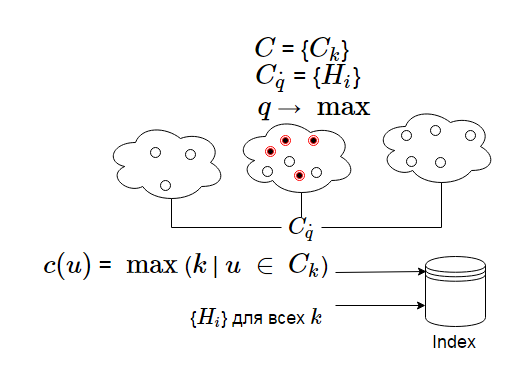
\includegraphics[scale=0.8]{pictures/index.png}}
  \end{center}
\end{figure}
\FloatBarrier

Стоит также сделать небольшое замечание, что некоторые соседние \textit{k-core} равны: $C_k = C_{k + 1}$. Нет смысла хранить их два раза, поэтому все повторяющиеся соседние \textit{k-core} мы будем хранить только один раз. Сейчас это кажется не очень хорошей оптимизацией, однако на реальных данных количество различных \textit{k-core} на несколько порядков меньше общего их количества, поэтому эта оптимизация имеет смысл. При описании дальнейших действий мы будем использовать переменную $h$~--- она означает количество различных \textit{k-core} в нашей ядерной декомпозиции, то есть количество \textit{k-core}, которые мы будем хранить в индексе.

Хранить ядерные индексы и набор компонент мы будем в соответствующих структурах данных (хеш-таблицах), позволяющих получать доступ к $c(v)$, набору всех компонент фиксированного \textit{k-core}, а также к компоненте фиксированного \textit{k-core}, в которой находится выбранная вершина $v$, за $O(1)$.

Однако мы до сих пор не сказали, как построить этот индекс. Строить его мы будем довольно просто: сначала построим набор компонент для $C_{k^*}$, а все остальные \textit{k-core} будем строить следующим образом: если уже построены \textit{k-core} порядков $k^*, k^*-1, \ldots, k$, то для построения \textit{$(k - 1)$-core} мы по одной добавим все вершины из $C_{k - 1} \setminus C_k$  и ребра, инцидентные им (благодаря свойству, что $C_{k - 1} \supseteq C_k$, этого достаточно), а затем обновим компоненты связности, которые благодаря новым вершинам могут объединиться в новые, более большие компоненты.

Эта фаза занимает $O(h \cdot |V(G)| + |E(G)|)$ времени, или же по-простому $O(hn + m)$, где $h$, напомним, количество различных \textit{k-core} в $G$. Однако эту асимптотику мы не будем учитывать в итоговом подсчете, потому что для каждого графа эта операция производится один раз, а затем построенный индекс используется для нахождения $C_Q^*$ и $H^*$.

Так как же найти $C_Q^*$ и $H^*$ по построенному индексу? На самом деле, очень просто. Так как $C_1 \supseteq C_2 \ldots \supseteq C_{k^*}$, то для нахождения \textit{k-core} наибольшего порядка, содержащего все вершины $Q$ в одной своей компоненте, мы можем использовать двоичный поиск по порядку \textit{k-core}. Чтобы проверить для фиксированного $C_k$, правда ли, что все вершины из $Q$ находятся в одной его компоненте, мы достанем из индекса информацию о компоненте для каждой вершины-запроса (напомним, что эта операция выполняется за $O(1)$), а затем проверим, что все эти числа получились одинаковые. Таким образом, проверка шага двоичного поиска происходит за $O(|Q|)$.

Суммируя все вышесказанное, получаем, что шаг нахождения $C_Q^*$ и $H^*$ выполняется за $O(|Q| \cdot \log(h))$.

\subsection{Фаза 2. Уменьшение размера $H^*$}

После выделения из графа $G$ \textit{k-core} $C_Q^*$ и его компоненты связности $H^*$, содержащей все вершины из $Q$, как мы уже отмечали, можно заметить, что $H^*$~--- ответ на нашу задачу, ведь степени всех его вершин хотя бы $k$ (то есть это \textit{k-core}), причем это $k$~--- максимально возможное (по построению $H^*$). Однако, не соблюдается одно оставшееся условие в постановке задачи~--- этот \textit{k-core} не минимального размера. Это мы и попытаемся исправить в этой и $3$-й фазах. Именно в этой фазе мы ставим перед собой следующую задачу: сейчас $H^*$ содержит все вершины-запросы, однако мы знаем, что среди них может быть шум. Задача этой фазы~--- выделить подграф, не содержащий шумовые вершины.

Напомним, что задача нахождения минимального по размеру \textit{k-core}~--- NP-полная. Какие эвристики мы можем применить? Первая мысль, которая приходит в голову~--- удалять слабо связанные вершины или подграфы из $H^*$, тем самым уменьшая его размер. Однако, так как степени всех вершин хотя бы $k$, сложно понять, какие вершины слабо связаны и удаление каких подграфов не нарушит свойство на степени вершины, то есть оставит подграф плотным. 

Нами был выбран обратный подход~--- добавление вершин. Будем строить итоговый подграф $H_{min}$ следующим образом: возьмем все вершины-запросы $Q$, удалим остальные вершины и ребра. Затем будем добавлять по одной вершине с некоторым приоритетом, тем самым постепенно увеличивая наш текущий подграф $H_{min}$. В каждый момент времени, когда текущий граф будет удовлетворять ответу на нашу задачу (то есть что компонента $H_{min}$, содержащая наибольшее количество вершин-запросов, содержит <<большинство вершин из $Q$>>, а также она довольно <<плотная>>), мы будем обновлять ответ. Понятно, что процесс не бесконечный~--- количество вершин в текущем ответе постоянно увеличивается, но подграф больше, чем $H^*$, мы не получим. Однако перед нами встает три глобальных вопроса:

\begin{enumerate}
  \item Какой выбрать приоритет для добавления вершин?
  \item Когда именно обновлять ответ (что такое <<большинство вершин из $Q$>>, что такое <<компонента довольно плотная>>)?
  \item Когда останавливать добавление вершин?
\end{enumerate}

\textbf{a. Какой приоритет использовать для добавления очередной вершины?}

Вариантов приоритета может быть множество. Однако давайте подумаем, что для нас важно в первую очередь. Во-первых, мы хотим, чтобы вершины, образующие сообщество (то есть набор вершин-запросов без шума), как можно быстрее объединились в связную компоненту и начали наращивать ее плотность. Для этого первым приоритетом сделаем количество компонент, которое объединяет вершина при добавлении. То есть, $p_1(v) = |A'| - |A|$, где $A$~--- множество компонент до добавления, а $A'$~--- после. Однако довольно часто при добавлении очередной вершины количество компонент остается неизменным. Что делать в этом случае? Так как для нас также важны степени вершин в итоговом подграфе, давайте акцентируем на этом внимание. При добавлении вершины $v$ степени вершин ее соседей, уже содержащихся в текущем подграфе, увеличиваются на $1$. Нам бы хотелось максимизировать это количество. Однако, нужно также учесть только что добавленную вершину и ее степень. Сделаем вторым приоритетом $p_2(v) = |N_{H_{min}}(v) \cap \{v \in V(H_{min}) | deg(v) < \mu(H^*)\}| - \max(0, \mu(H^*) - |N_{H_{min}}(v)|)$, где $N_{H_{min}}(v)$~--- множество вершин из $H_{min}$, соединенных с $v$ ребром. Другими словами, мы учитываем со знаком плюс количество вершин-соседей вершины $v$ из $H_{min}$, степень вершин которых еще меньше требуемой $\mu(H^*)$, а со знаком минус учитываем количество ребер, которое не хватает только что добавленной вершине до требуемой степени $\mu(H^*)$.

\textbf{b. Что же такое <<большинство вершин из $Q$>>, что значит <<компонента довольно плотная>>?}

Мы будем говорить, что подграф $H \subset G$ содержит большинство вершин из $Q$, если количество вершин-запросов в нем хотя бы $\alpha(|Q|) \cdot |Q|$. $\alpha(|Q|) \in (0, 1]$ или просто $\alpha$~--- некий коэффициент, зависящий от количества вершин-запросов. Какие же значения должно принимать $\alpha$? С одной стороны, мы хотим, чтобы <<большинство вершин>> было действительно большинством, поэтому мы будем считать, что шума в запросе меньше $\frac{|Q|}{2}$ (то есть $\alpha \ge 0.5$). С другой стороны, даже $\frac{|Q|}{2}$ вершин почти всегда слишком много для шума.  

Нас также интересует, что значит <<компонента довольно плотная>>. Будем говорить, что компонента довольно плотная, если в ней достаточно много ребер (то есть и плотность достаточно большая). Для выбора границы количества ребер было попробовано несколько функций, оптимальной оказалось следующая: $|E(H_{min})| \ge (V(H_{min}) - |Q|) \cdot \mu(H^*) + \beta(|Q|) \cdot |Q|)$, то есть у всех вершин-запросов степень вершин берется равной $\beta$ (еще один параметр), а у остальных она должна быть хотя бы $\mu(H^*)$ (на самом деле, если в запросе есть шум, степень вершины должна быть больше, однако, если шума нет, это неправда). 

На самом деле, условие на плотность компоненты можно не учитывать, а просто проверять, что текущий подграф содержит <<большинство вершин из $Q$>>~--- ведь в зависимости от этих условий мы только решаем, обновлять ли ответ. Однако, условие на плотность компоненты было добавлено с целью уменьшения количества обновлений ответа и уменьшения времени работы алгоритма.

Для выбора оптимальных значений параметров $\alpha$ и $\beta$ по фиксированному $|Q|$ было решено провести исследование. Исследование проводилось на тех же экспериментах, что и сравнение различных алгоритмов (об этом подробнее в главе $3$). Результаты исследований приведены в таблице ниже ($k$~--- порядок \textit{k-core}, то есть $k = \mu(H^*)$).

\begin{table}[!h]
\centering
\caption{Оптимальные значения параметров $\alpha$ и $\beta$ для различных $|Q|$}\label{parameters-research}
  \begin{tabular}{| l | l | p{1cm} |}
  \hline
  $|Q|$ & $\alpha$ & $\beta$ \\\hline
  2   & 1      & 1        \\\hline
  3   & 2 / 3  & 1        \\\hline
  4   & 1 / 2  & 1        \\\hline
  5   & 3 / 5  & 2        \\\hline
  6   & 2 / 3  & 2        \\\hline
  7   & 4 / 7  & 3        \\\hline
  8   & 3 / 4  & 3        \\\hline
  > 8 & 7 / 10 & 4        \\\hline
  \end{tabular}
\end{table}
\FloatBarrier

\textbf{c. Когда останавливать алгоритм добавления?}

Понятно, что остановить его можно, когда мы например добавили все вершины из $H^*$. Однако, так как размер $H^*$ может быть достаточно большим, это не самое оптимальное решение~--- после того, как наш подграф станет связным, он уже будет содержать все вершины-запросы, а следовательно и весь шум, в то время как наша задача как раз от него избавится. Поэтому будем останавливать алгоритм, когда все компоненты объединились в одну, то есть текущий подграф стал связным.

\begin{figure}[!h]
\caption{Пример работы фазы $2$}\label{phase2-example}
\centering
  \begin{center}
    \makebox[\textwidth]{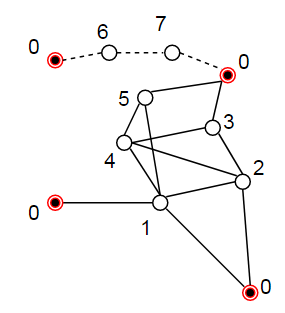
\includegraphics[scale=1.2]{pictures/phase2.png}}
  \end{center}
\end{figure}

Например, пусть $H^*$ выглядит так, как на рисунке~\ref{phase2-example} (таким он взят для упрощения и более простого объяснения и понимания написанного выше текста). Вершины-запросы в нем отмечены красным, их мы возьмем первыми (шаг $0$). Затем будем добавлять вершины по одной, в порядке, как показано на рисунке: сначала добавляем вершину $1$, потому что она объединяет две компоненты, затем $2$, потому что у нее максимальный второй приоритет, и т.д. Закончим мы, когда $H_{min}$ станет связным, то есть в данном случае, когда мы добавим все его ребра. Однако, оптимальным ответом будет подграф, не содержащий пунктирные ребра, потому что он более плотным. И, как мы видим, действительно, не добавленная вершина~--- явный шум, добавлять ее в ответ не стоит.

\subsection{Фаза 3. Восстановление условия на степень вершин}

После того, как мы выполнили фазу $2$, мы нашли подграф, который будем обозначать $H_{min}^*$. Этот подграф можно было бы вернуть как ответ, но, как мы только что видели на рисунке~\ref{phase2-example}, вполне может оказаться, что $H_{min}^*$ далек от идеального ответа. Почему? Ведь мы добавляли вершины по одной с, как нам казалось, оптимальным приоритетом. На самом деле, так как в первую очередь мы стремимся добавлять вершины, которые лучше всего объединяют наши текущие компоненты, и следим за степенями вершины только во вторую очередь (при этом фактически мы только пытаемся удовлетворить условие на степени вершин, но это не факт, что точно получится), ответ может получиться неоптимальным. Поэтому с $H_{min}^*$ надо что-то сделать, чтобы удовлетворить условие на степени вершин.

Сейчас может показаться, что фаза $2$ была вообще лишней, ведь мы из \textit{k-core}, который достаточно плотно связан благодаря условиям на степени вершин, сделали что-то непонятное, казалось бы только хуже. Это не так, потому что во-первых исходный $H^*$ содержал все вершины-запросы, в том числе шум, а подграф-ответ может быть намного плотнее. Во-вторых, это только временно, сейчас мы применим несколько эвристик и подграф станет плотным \textit{k-core} б\'{о}льшего порядка.

Для начала давайте удалим слабо связанные вершины. Так как теперь наш подграф не \textit{k-core}, мы можем предложить логичные условия для этого. Вспомним про наш введенный параметр $\beta$, который отвечал за минимальные степени вершин-запросов. Давайте удалим все вершины-запросы, имеющие степень меньше $\beta$, то есть не подходящие под наше описание (такие вершины могли остаться, потому что мы смотрели только на общее количество ребер подграфа, а не на степени вершин).

После удаления слабо связанных вершин-запросов выполним еще раз фазу $1$ уже на оставшихся запросах. На самом деле, всю фазу нам выполнять не нужно, от этой фазы нам нужно только новое значение $k^{opt}$~--- наибольший порядок \textit{k-core}, в котором все оставшиеся вершины-запросы лежат в одной компоненте связности.

Теперь мы сделаем главный шаг этой завершающей фазы. Его идея заключается в следующем: возьмем все оставшиеся выделенные вершины и найдем минимальное количество не выделенных, которые их соединяют. То есть, взяв множество оставшихся выделенных вершин $Q' \subseteq Q$, мы хотим найти такое множество вершин $V_{opt} \subseteq V(H_{min}^*) \setminus Q'$ минимального размера, что $G[V_{opt} \cup Q']$~--- связен (напомним, $G[V]$~--- подграф, порожденный множеством вершин $V$). Это даст нам <<каркас>> подграфа $H_{min}^*$, который мы сможем после этого нарастить, почти как в фазе $2$.

То, что мы описали выше~--- ничто иное как задача Штейнера. Оригинальная задача Штейнера звучит так: по данному взвешенному графу $G$ и выделенным в нем множеству вершин $Q$, найти минимальное остовное дерево на этих вершинах. Занимательный факт состоит в том, что если $|Q| = 2$, то задача сводится к кратчайшему пути в графе, если $|Q| = |V(G)|$, то задачу сводится к построению минимального остовного дерева в графе, но если оба этих условия не выполняются, задача становится NP-полной. Можно отметить, что в нашей задаче граф не взвешенный, однако задача Штейнера остается NP-полной даже в случае, когда все веса в графе одинаковые. Задача Штейнера была давно изучена, и в статье Kou et al. \cite{Kou81} был представлен оптимальный алгоритм ее решения с аппрокцимацией $2 - \frac{2}{|Q|}$ и доказательством того, что за полиномиальное время задачу Штейнера нельзя решить лучше. Мы воспользуемся решением из этой статьи и применим его к нашей задаче.

Найдя искомый <<каркас>>, применим к нему слегка измененную фазу $2$. Во-первых, каркас уже связен и нам не нужен приоритет на количество объединенных компонент. Во-вторых, хотелось бы усовершенствовать эту фазу, чтобы строго гарантировать плотность итогового подграфа. Поэтому мы меняем фазу $2$ следующим образом:

\begin{enumerate}
  \item Добавлять вершины будем только по второму приоритету (на самом деле, можно оставить и первый, просто он не будет нести никакого смысла);
  \item Останавливаться будем, когда минимальная степень вершины станет хотя бы $k^{opt}$, ведь мы точно знаем, что на оставшихся вершинах-запросах можно построить \textit{$k^{opt}$-core};
  \item Мы не будем по ходу добавления вершин обновлять ответ, ответом будет просто финальный подграф.
\end{enumerate}

Изменив фазу $2$ описанным выше образом, мы запускаем ее на $H_{min}^*$ с удаленными слабо связанными вершинами-запросами и получаем итоговый ответ на задачу.

\begin{figure}[!h]
\caption{Пример работы фазы $3$}\label{phase3-example}
\centering
  \begin{center}
    \makebox[\textwidth]{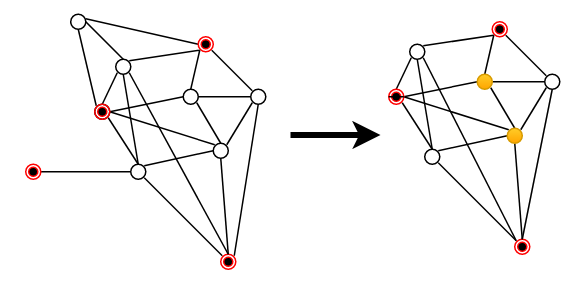
\includegraphics[scale=1.0]{pictures/phase3.png}}
  \end{center}
\end{figure}

Работа этой фазы представлена на рисунке~\ref{phase3-example}, где исходный подграф $H_{min}^*$ (который до фазы $2$ являлся \textit{3-core})находится слева, а полученный после обработки~--- справа. Сначала мы удалили явно слабо связанную вершину-запрос, а затем выделили с помощью задачи Штейнера две желтые вершины, связывающие $3$ оставшихся запроса и образующих тем самым <<каркас>> из $5$ вершин. После этого мы запускаем измененную фазу $2$ и получаем ответ, представленный справа на рисунке. Как видно, он получился меньше и плотнее, а также является \textit{4-core} вместо \textit{3-core}.

\section{Теоретическая оценка качества}

Сложно оценивать качество алгоритма без проверки на практических данных. Однако в этом разделе мы отметим несколько явных преимуществ по сравнению с имеющимися алгоритмами.

\begin{itemize}
  \item Наш алгоритм учитывает шум в запросе, если он есть и его меньше половины, а также требует наличие всех вершин в запросе, если явного шума нет;
  \item Наш алгоритм должен работать не хуже Barbieri et al. \cite{Barbieri15}, потому что мы в итоге находим \textit{k-core} порядка хотя бы $\mu(H^*)$. Наш алгоритм может работать хуже из-за отличающейся эвристики, однако на запросах с шумом мы должны находить \textit{k-core} с б\'{о}льшим порядком, а следовательно плотнее;
\end{itemize}


\section{Literature}

\begin{itemize}
    \item 1  Gionis A., Mathioudakis M., Ukkonen A. Bump hunting in the dark: Local discrepancy maximization on graphs // 2015 IEEE 31st International Conference on Data Engineering (ICDE). — 2015. — Т. 978. — С. 1155–1166.
    \item 2  Faloutsos C., McCurley K. S., Tomkins A. Fast discovery of connection subgraphs // Proceedings of the tenth ACM SIGKDD international conference on Knowledge discovery and data mining. — 2004. — Т. 1. — С. 118–127.
    \item 3  Faloutsos C., Tong H. Center-Piece Subgraphs: Problem Definition and Fast Solutions // Proceedings of the 12th ACM SIGKDD international conference on Knowledge discovery and Data Mining. — 2006. — Т. 1. — С. 404–413.
    \item 4  The Minimum Wiener Connector Problem / N. Ruchansky [et al.] // Proceedings of the 2015 ACM SIGMOD International Conference on Management of Data. — 2015. — Т. 1. — С. 1587–1602.
    \item 5  Efficient and effective community search / N. Barbieri [et al.] // Data Mining and Knowledge Discovery. — 2015. — Т. 29. — С. 1406–1433.
    \item 6  Zhu L., Ng W. K., Cheng J. Structure and attribute index for approximate graph matching in large graphs // Journal Information Systems. — 2011. — Т. 36. — С. 958–972.
    \item 7  Robust local community detection: on free rider effect and its elimination / Y. Wu [et al.] // Journal Proceedings of the VLDB Endowment. — 2015. — Т. 8. — С. 798–809.
    \item 8  Approximate closest community search in networks / X. Huang [et al.] // Proceedings of the VLDB Endowment. — 2015. — Т. 9. — С. 276–287.
    \item 9  Sozio M., Gionis A. The community-search problem and how to plan a successful cocktail party // Proceedings of the 16th ACM SIGKDD international conference on Knowledge discovery and data mining. — 2010. — Т. 978. — С. 939–948
    \item 10 Local search of communities in large graphs / W. Cui [et al.] // Proceeding SIGMOD ’14 Proceedings of the 2014 ACM SIGMOD International Conference on Management of Data. — 2014. — Т. 978. — С. 991–1002.
    \item 11 Mining Connection Pathways for Marked Nodes in Large Graphs / L. Akoglu [et al.].
\end{itemize}


\end{document}